\section{VLANs}
Ein physisches Netz wird in mehrere logische Teilnetze (Layer 2) unterteilt.

\begin{table}[H]
	\begin{tabular}{l|l}
		\multicolumn{1}{c}{Vorteile} & \multicolumn{1}{c}{Nachteile} \\
		\hline
		Kosten & (Konfiguration) \\
		Security &  \\
		Flusskontrolle &  \\
		Übersicht &  \\
		kleinere Broadcast-Domain &  \\
		Effizienz \& Performance & 
	\end{tabular}
\end{table}

\textbf{Arten von VLANs}
\begin{itemize}
	\item Daten VLANs
	\item Default VLAN (bei cisco 1)
	\item Voice VLAN
	\item Management VLAN
	\item Native VLAN (Frames ohne VLAN-Tag kommen in das Native VLAN, kann nur am Trnk passieren)
\end{itemize}

Access Ports transportieren nur ein VLAN. \\
Trunk Ports können viele VLANs transportieren. \\
Die VLAN-Namen werden zusätzlich im Header eingetragen (802.1q $\rightarrow$ Ethernet)

\textbf{ACL} \\
Je nach IP-Adresse (Standard) bzw. Port (Extended) wird ein Packet blockiert oder zugelassen.

\textbf{Wildcardmask} \\
Subnetzmaske: Teilt IP-Adresse in Netz- und Hostteil \\
1 ... Netzteil (relevant für das Netz) \\
0 ... Hostteil (irrelevant für das Netz) \\
$\rightarrow$ unflexibel

Wildcardmaske '1' \& '0' können beliebig gezählt werden \\
0 ... relevantes Bit der IP-Adresse \\
1 ... nicht relevantes Bit der IP-Adresse

\begin{tabbing}
	255.255.255.255 ~~~ \= any \\
	0.0.0.0 ~~~~~~~~~~~~~~~ \= host
\end{tabbing}

\textbf{Position der Wildcardmask}
\begin{figure}[H]
	\centering
	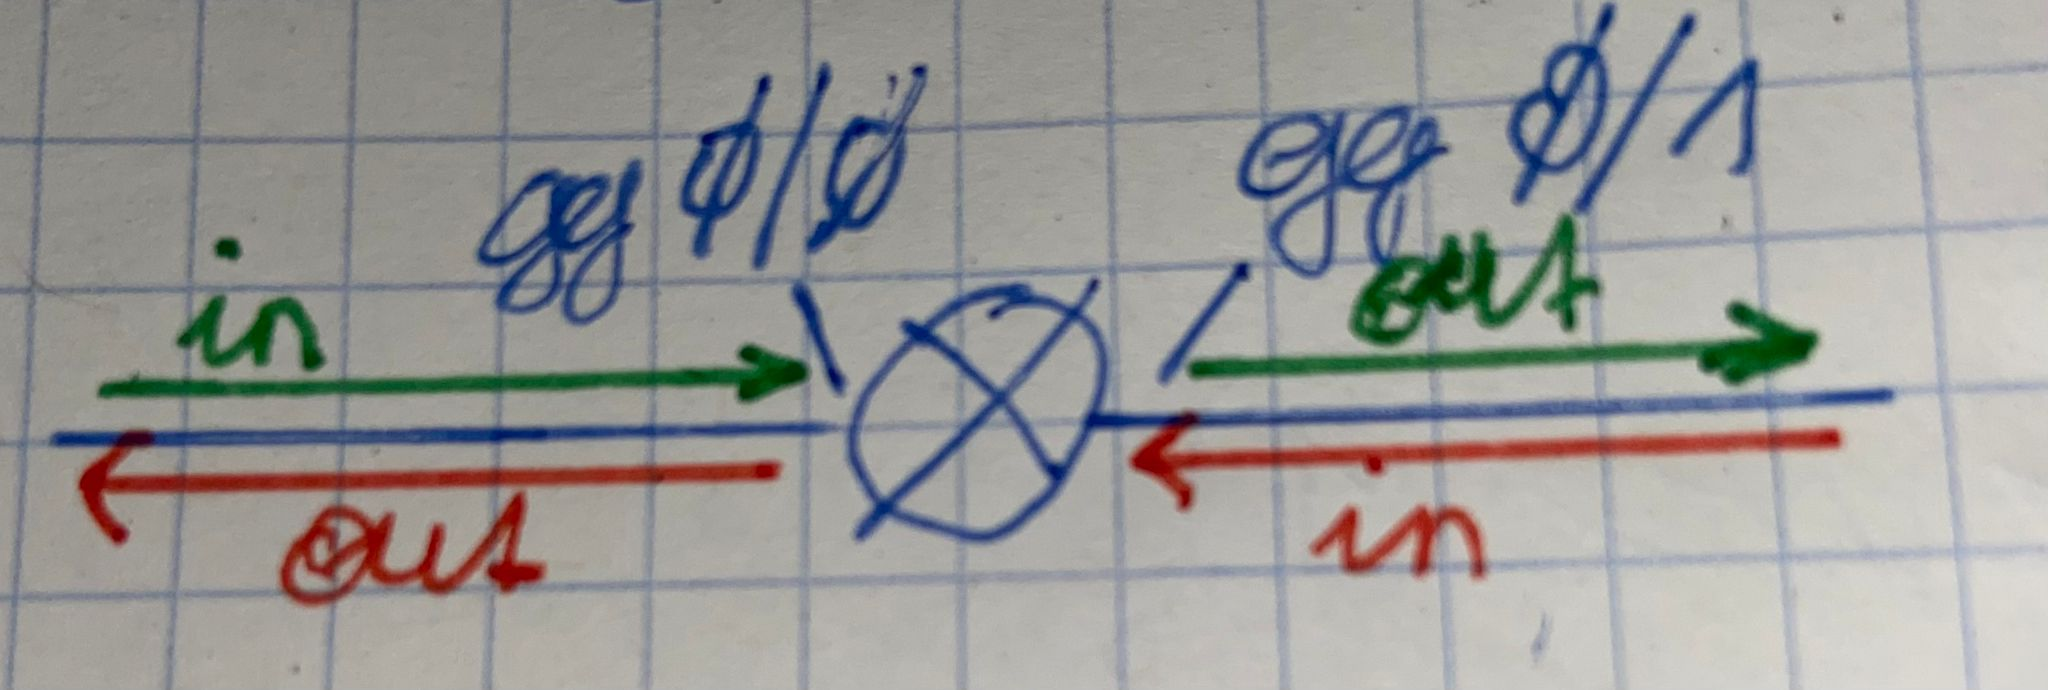
\includegraphics[width=0.8\linewidth]{figures/wildcard.jpeg}
	\caption{Position der Wildcardmask}
\end{figure}

Regeln bei Interfaces: eingehend \& ausgehend \\
\textbf{Achtung} Die letzte Zeile in jeder ACL ist 'deny any'.

\textbf{Static NAT (1:1 Mapping)} \\
\begin{figure}[H]
	\centering
	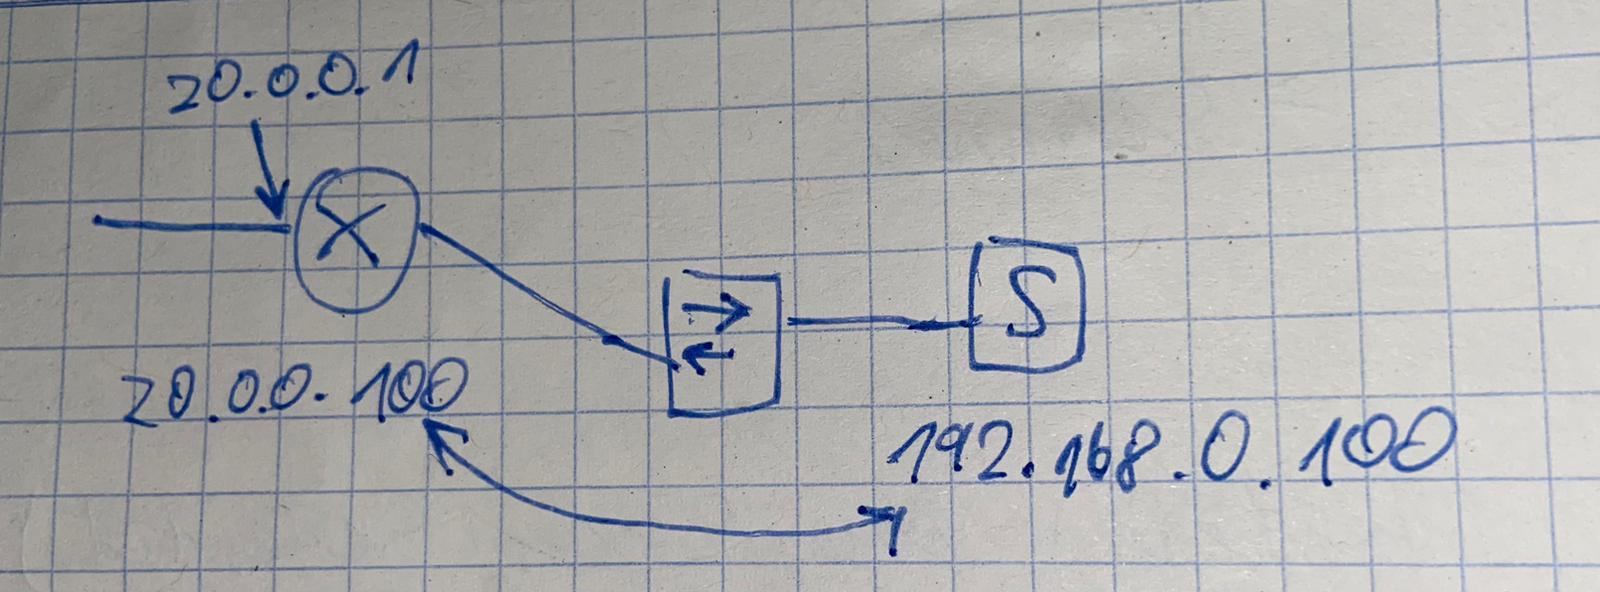
\includegraphics[width=0.8\linewidth]{figures/static_nat.jpeg}
	\caption{Static NAT, 1:1 Mapping}
\end{figure}

\textbf{NAT mit PAT (n:1 Mapping)}
\begin{figure}[H]
	\centering
	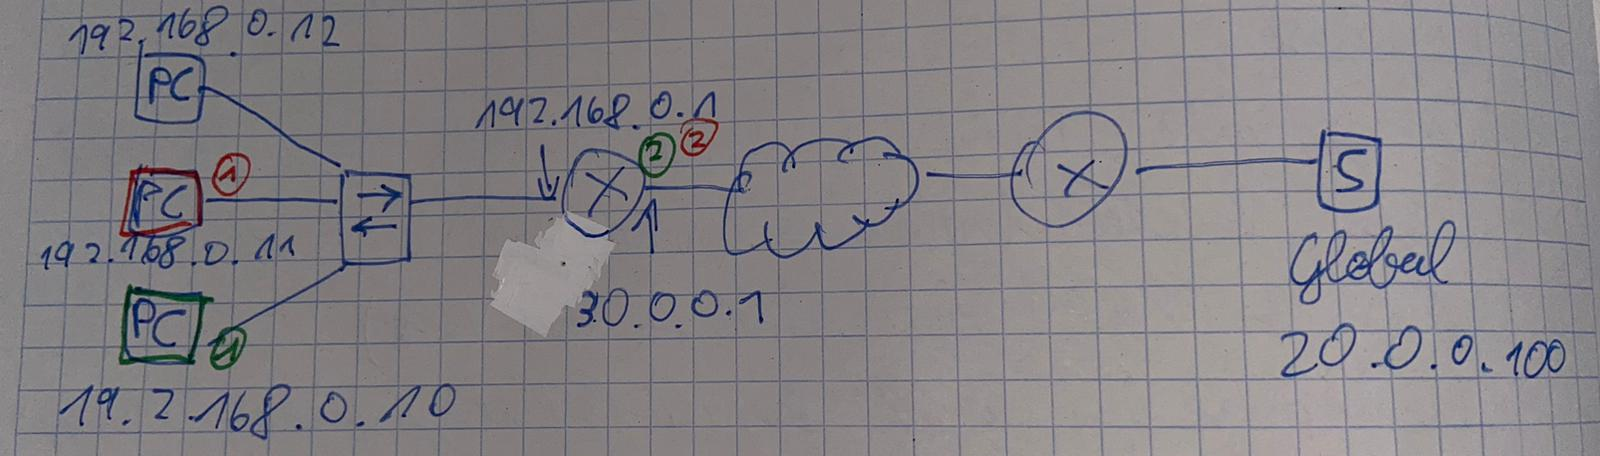
\includegraphics[width=0.8\linewidth]{figures/pat_nat.jpeg}
	\caption{NAT mit PAT, n:1 Mapping}
\end{figure}

\begin{table}[H]
	\begin{tabular}{c|cccc}
		& Source IP & Destination IP & Source Port & Destination Port \\
		\hline
		{\color[HTML]{32CB00} 1} & 192.168.0.10 & 20.0.0.100 & 51000 & 443 \\
		{\color[HTML]{FE0000} 1} & 192.168.0.11 & 20.0.0.100 & 51000 & 443 \\
		{\color[HTML]{32CB00} 2} & 30.0.0.1 & 20.0.0.100 & 51000 & 443 \\
		{\color[HTML]{FE0000} 2} & 30.0.0.1 & 20.0.0.100 & 51001 & 443
	\end{tabular}
\end{table}

\begin{table}[H]
	\begin{tabular}{l|l}
		\multicolumn{1}{c}{Vorteile} & \multicolumn{1}{c}{Nachteile} \\
		\hline
		\textbf{+ IP-Adressen sparen} & \textbf{- Ende zw. Ende Verbindung geht verloren} \\
		+ Security & - Paketverfolgung und Troubleshooting \\
		+ IP-Adressen Schema kann frei gewählt werden & - Performance \\
	\end{tabular}
\end{table}

